\chapter{基于一致性预测的高超声速飞行器轨迹预测}\label{chap:cp-HFV}
上一章中我们介绍了基于强收敛模式下一致收敛的统计学习理论给出的结论是断言, 并且同时Vapnik指出统计学习理论属于现象学学习模型\citep{vapnik2020,Husserl1937,wangdefeng-xianxiangxue-2005}. 通过现象学学习理论我们已经知晓学习机器的输出是一个暴力得分\citep{vapniktalk2015}. 对于“暴力得分”朴素的理解即是说学习过程需要大量样本(这一点通过第 \ref{chap:edbed} 章介绍的学习理论的一般原则亦能说明)而并不像人类学习一样需要少量样本; 但更切近地说来, 真正意义上的“暴力”是我们通过现象学还原的方法澄明了的, 即在现象学的视野下所谓“暴力得分”背后的事情本身乃在于对“异化”的理解, 即由诸样本建构生成的少数支持向量现在反过来支配大量样本. 而究其在技术层面的理解, 就如Chervonenkis也明确指出的, 学习理论的输出的确没有任何概率可言, 它仅仅就是一个暴力得分函数, 我们仅仅只能根据其得到分类的标识而不能据此展开任何可信程度的度量 \citep[p. 22]{2006Hedging}. 

机器学习研究者们是完全知晓我们仅能根据SVMs输出实现分类而不能展开可信度判断这一事实的. 也就是说我们是不能够根据输出得分的取值进行任何概率意义上的比较或者决策的评判, 机器学习算法的输出仅能用于类别标记. 正因为如此, 就提出多种校正的方法以期将暴力得分“软化”为概率意义上的取值. 在众多校正方法中最有名的就是Platt方法, 这种校正方法也是目前各种开源软件包中默认采用的方法 \citep{Platt1999}. 但是仔细看来, 也正如Vapnik所言Platt校正方法把SVMs退化为模型驱动的方法 \citep{Vapnik2021}. 本来借助Vapnik提出的SVMs方法, 经验数据获得了其超越表征——这是真正意义上的数据驱动,  然而Platt重新通过假设这些输出函数服从Sigmoid函数而将原本纯粹数据驱动算法重新退化为模型驱动算法, 同时也将现象学学习理论重新拉入知性科学的框架中去了 \citep{Vapnik-Synergy-2016}.

这样一来, 我们就仍然不得不面对这样一个事实, 即真切地说来, 我们无法基于机器学习算法的输出——就是那暴力得分函数本身——\textsf{为单个具体的对象}做出任何可信的判断. 而现在我们所要面临的问题恰恰就是需要为机器学习算法的\textsf{单个输出}提供一种可信度量. 并且真正说来, 如果能为单个个体提供有效的不确定度量, 那么有限整体的不确定控制难道不就是自明的吗? 针对这一问题的解决, 最早就是由 \citet{soton1999} 和 \citet{Saunders1999} 提出并解决的. 1996年夏天伦敦大学皇家霍洛威学院 Alexander Gammerman、Vladimir Vovk 邀请 Vladimir Vapnik举办了一系列机器学习研讨会, 讨论的主题主要就聚焦在Vapnik的支持向量机方面的工作, 也就是在那个时候他们意识到学习机器中支持向量的数量可以用作对冲预测(hedged prediction)来为单个样本提供可信程度的度量. 

最初的一致性预测(Conformal Prediction)思想就是基于Vapnik提出的SVMs思想 \citep{gammerman1998}. 有关Conformal Prediction核心思想的提出, Vladimir Vovk自己承认\citep{vovk-harris-Gammerman2015}, 早在1966年Chervonenkis就意识到对于给定的样本序列$x_{1}, \ldots, x_{l}$, 如果我们给此序列添加一个样本$x_{l+1}$进去, 然后利用新的样本序列$x_{1}, \ldots, x_{l}, x_{l+1}$来构建广义肖像法\citep{vapnik1963}; 当基于新序列构建好广义肖像法后, 把新添加的样本$x_{l+1}$移除, 那么当且仅当$x_{l+1}$样本是支持向量的时候, 构建好的广义肖像法才会发生改变. 换言之, 如果新添加的样本$x_{l+1}$不是支持向量, 那么此时的广义肖像法模型就具有稳定的学习推广能力. 但问题则在于那最后添加进来的向量$x_{l+1}$是支持向量的概率是$\frac{k}{l+1}$, 其中这里的$k$是支持向量的数量, $l$是样本量. 并且在通常的情形下支持向量数目$k$是不会超过VC维. 换言之, 从另一个方面而言, 也就是说如果新添加的样本$x_{l+1}$不是支持向量, 那么当我们在样本序列$x_{1}, \ldots, x_{l}$上得到的学习模型在新的样本序列$x_{1}, \ldots, x_{l}, x_{l+1}$上也就不会出错. 因此, 这样一来在长度$l$的样本上学习模型犯错数目的数学期望就将不会超过
\begin{align*}
\frac{n}{l+1}.
\end{align*}
这也就是说为什么最后学习模型——当然尽管这种学习模型只仅限于广义肖像法——会显示出其仅仅依赖于VC维而并不依赖于空间的维数. 但是当时Vapnik建议不要发表这个发现, 因为在Vapnik看来, 这太简单了, 所以这个结果一直到1974年他们合著的著作 \citep{vapnik1974} 中才得以首次发表 \citep{Alexey2015}. 

先前在算法随机理论(algorithmic theory of randomness)工作了相当长时间的Vovk意识到Chervonenkis早期的观点可以用于开展对冲预测模型. Vovk注意到我们可以将数量较少的那些支持向量转译为某种置信预测. 简单说来是这样一种情形, 即我们考虑的分类问题 ($|\mathbf{Y}|$有限)可以从算法随机理论的角度看待这一问题, 那就是说对于随机原序列$z_{1}, \ldots, z_{l}$\footnote{在这里我们将数据对$(x, y)$记为$z$.}, 如果仅仅一个可能的扩展$z_{1}, \ldots, z_{l}, (x_{n}, y), y \in \mathbf{Y}$的算法随机性的衰减是微量的, 那么在给定序列$z_{1}, \ldots, z_{l}$时, 我们就可以为新对象$x_{n+1}$的标签$y_{n+1}$给出一个置信预测.

真正说来, 一致性预测最初的出发点是服务于超越推理(Transductive Inference)的. 结合算法随机理论和超越推理, 考虑在线预测模式: 即对于每次试验$n = 1, 2, \ldots$, 给定前$n-1$个观测$(z_{1}, \ldots, z_{n-1})$, 我们想知道第$n$个观测的内容是什么. 通常而言, 这些观测都被视为由两部分组成, 即他们的对象$x$和标签$y$. 我们想要做的是给定第$n$个对象$x_{n}$来预测其标签$y_{n}$. 这些所有的观测都被假设是由相同但未知的概率分布函数独立地生成的——在面对具体问题时更多地会通过随机抽取样本来通过技术满足此假设的实现. 

一致性预测考虑给出的是区域预测, 即预测算法要求输出第$n$个观测的所有可能的结果. 统计学最近的研究已经表明, 在统计学框架下所得到的p-值始终无法获得有效的估计(参见\citep{Ioannidis2005,Taylor2015,Tibshirani2015,Wasserstein2016,Altman2017,Andrade2019,Betensky2019,Lee2019,Ioannidis2019}); 然而, 对于一致性预测(最初命名为\textsf{超越置信机}(\textit{Transductive Confidence Machines})), p-值有效的要求是自动满足的. 也就是说我们基于一致性预测得到的p-values——其实应该被称作是p-functions——是自动满足有效要求的. 这样一来, 当我们给定“显著性水平”$\epsilon$, 一致性预测出错的频率是严格受到控制的, 并且如果随机性假设被满足——比如我们用技术手段随机化样本数据——那么犯错的频率是被精确控制的. 更甚者(这是相对统计学而言), 此算法得到的p-值自动有效的校正是无需任何分布假设(因为底层现代机器学习算法(以SVMs为例)无需分布假设), 所以一致性预测输出的结果都是断言而不是应诺.


\section{一致性预测理论介绍}
现在我们形式化介绍一致性预测. 考虑机器学习中的分类问题, 基于观测样本空间我们的目的是为新观测对象$x_{n}$预测其真实标签$y_{n}$. 

对于任意样本序列$(x_{1}, y_{1}), \ldots, (x_{n-1}, y_{n-1}) \in \mathbf{Z}^{*}$ 以及任意的新对象$x_{n} \in \mathbf{X}$, 机器学习算法给出的结果可以表述为下列映射关系:
\begin{align}
\label{simple-prediction}
D: \mathbf{Z}^{*} \times \mathbf{X} \rightarrow \mathbf{Y}.
\end{align}
我们将这样的机器学习算法称作是\textsf{简单预测}(\textit{simple predictor}). 此函数为新对象$x_{n}$给出暴力得分得到的预测标签$y_{n}$.

现在我们需要的工作是为此暴力标签给出一个“软化”操作, 即我们想为暴力标签补充提供到底其可信程度是多少, 然后再尝试提供一个在指定显著水平下的“区间估计”, 即输出某集合估计结果. 一致性预测基于提前给定的显著性水平$\epsilon \in (0, 1)$, 新对象的\textsf{置信预测}$\Gamma$可以表述为下列形式:
\begin{align}
\label{confidence-predictor}
\Gamma: \mathbf{Z}^{*} \times \mathbf{X} \times (0, 1) \rightarrow 2^{\mathbf{Y}}
\end{align}
其中, 这里$2^{\mathbf{Y}}$是类别集合$\mathbf{Y}$的势 (power of set).

置信预测$\Gamma$的输出结果
\begin{align}
\label{confidence-output}
\Gamma^{\epsilon}(x_{1}, y_{1}, \ldots, x_{n-1}, y_{n-1}, x_{n})
\end{align}
必须满足下列关系式
\begin{align}
\Gamma^{\epsilon_{1}}(x_{1}, y_{1}, \ldots, x_{n-1}, y_{n-1}, x_{n}) \subseteq \Gamma^{\epsilon_{2}}(x_{1}, y_{1}, \ldots, x_{n-1}, y_{n-1}, x_{n})
\end{align}
其中这里的$\epsilon_{1} \geq \epsilon_{2}$. 在置信水平$1 - \epsilon$下, 置信预测$\Gamma$宣布新对象的标签$y_{n}$在其预测集合中, 即
\begin{align}
\label{confidence-y}
y_{n} \in \Gamma^{\epsilon}(x_{1}, y_{1}, \ldots, x_{n-1}, y_{n-1}, x_{n}).
\end{align}

如果置信预测$\Gamma$的预测集合不包含任何标签, 我们称之为空元素集合预测; 如果置信预测$\Gamma$的预测集合只包含一个标签(并不需要必须要求此标签就是真实标签)我们就称之为单元素集合预测; 如果置信预测$\Gamma$的预测集合包含多个标签, 我们称之为多元素集合预测. 如果真实标签$y_{n}$不被以上三种预测结果所包含, 那么我们就称置信预测$\Gamma$输出错误预测. 因此, 这样说来对于多元素集合预测, 如果输出结果为多元素但是包含真实标签, 我们并不视这种情形为预测错误, 这仅仅表明置信预测$\Gamma$并没有提供高效的信息而已. 

置信预测$\Gamma$具有两个显著的特征: \textsf{置信度}和\textsf{可信度}. 其中置信度表征预测的\textsf{有效性} (validity), 可信度表征预测的\textsf{高效性} (efficiency). 给定显著性水平 $\epsilon$, 如果预测错误的相对频率在任意给定的显著性水平$\epsilon$下不超过$\epsilon$, 我们就认为这样的预测是有效的. 这就意味着在用户指定的任意显著性水平下机器都能够给出有效的预测结果. 而对于可信度则意味着我们希望预测结果能给出更多信息的预测. 显然, 我们希望预测集合在尽可能包含真实标签的同时集合元素的个数越少越好, 这就意味着置信预测给出的结果是高效的. 

对于这两个性质, 如果我们就一致性预测方法和传统统计学方法而言, 很显然这是一种革命, 这是因为
\begin{enumerate}
\item 一致性预测方法不需要分布假设, 而统计学的几乎所有统计推断都依赖于分布假设. 也正是基于这一点, 北美统计系培养的新一代研究人员创造了一个新词: 无模型假设的不确定性量化 (Distribution-Free Uncertainty Quantification, DFUQ)\footnote{\url{https://sites.google.com/berkeley.edu/dfuq-22/home}}.
\item 一致性预测方法处理的非渐近问题, 而统计学的几乎所有统计推断都依赖于渐近假设.
\item 一致性预测方法提供的是单个个体的不确定性量化, 不关注总体量化指标——因为当个体不确定性被控制住后, 总体的结果是必然的.
\end{enumerate}

如果我们就机器学习算法而言, 一致性预测的确能够为任意的机器学习算法提供可信的不确定性度量. 这是因为一致性预测方法是以机器学习算法的输出——正就是本质为暴力得分的输出——作为开端的. 因此, 一致性预测方法也被视作是可信机器学习算法的一种完整的实现. 但我们需要明确的是, 就一致性预测的这两个性质本身而言——正如我们已经提示过的——其条件都建立在数据服从独立同分布假设或者更弱一些的可交换性假设.

在继续阐述一致性预测之前我们需要引进一个新的概念: “袋子”. “袋子”也称作是“多元素集合”, 即在“袋子”中的元素是忽略顺序——这一点与“集合”是相同的; 与此同时“袋子”允许出现完全一样的元素——这一点与集合不一样. 容量为$n$的“袋子”指的是“袋子”中的元素的个数为$n$, 并记做 $\Lbag z_1, \ldots, z_{n} \Rbag$. 记$\mathbf{Z}^{(n)}$为来自可测空间$\mathbf{Z}$中的$n$个元素组成的大小为$n$的所有“袋子”的集合. 记 $\mathbf{Z}^{*}$是可测空间$\mathbf{Z}$的所有元素的所有“袋子”的集合. 这样一来, 一致性预测的思想就是——基于算法随机理论——需要基于某非一致度量函数(nonconformity measure)来量测新数据$(x_{n}, y)$与已知样本序列$\Lbag z_1, \ldots, z_{n-1} \Rbag$的符合程度. 我们需要将待估标签的所有可能都按照这种方式计算, 进而得到每个候选标签对应的非一致性得分(nonconformity score). 通过对非一致得分的标准化我们就得到每个候选标签对应的p-值.

就一致性预测的历史来看, \textsf{非一致性测度}的根基是来源于SVMs中拉格朗日乘子$\alpha_{i}$. 因为我们从现象学角度阐述SVMs后就会明白, 拉格朗日乘子$\alpha_{i}$表征的是样本的异化程度:
\begin{enumerate}
\item 如果样本$z_{i}$对应的$\alpha_{i} = 0$, 那么表明样本$z_{i}$的异化程度最低, 这样的样本就都是经典的、平凡的;
\item 如果样本$z_{i}$对应的$\alpha_{i} = C$(这里的$C$是$\alpha$的最大取值), 那么表明样本$z_{i}$的异化程度最高, 这样的样本就是最极端、最野样本;
\item 如果样本$z_{i}$对应的$0 < \alpha_{i} < C$, 那么表明样本$z_{i}$的异化程度就介于平凡和极端之间.
\end{enumerate}

面对越极端的样本, 我们就越有信息给出其类别标签. 因此, 非一致性测度就是评估新样本与旧样本异化程度的方法, 或者评估新样本与旧样本“有多么奇怪”. 非一致性测度将每个可能的新样本和“袋子”中旧样本映射为一个数值得分, 即非一致性得分.
\begin{align}
\label{nonconformity-score}
A: \mathbf{Z}^{*} \times \mathbf{Z} \rightarrow \mathbf{R}.
\end{align}
我们对样本中的每个样例都执行非一致性测度, 就可以得到对于每个样本$n = 1, 2, \ldots$定义的诸非一致性测度$A_{n}$的集合
\begin{align}
\label{nonconformity-set}
A_{n}: \mathbf{Z}^{n-1} \times \mathbf{Z} \rightarrow \mathbf{R},
\end{align}
其中这里$n$是“袋子”的大小. 因此, 对于“袋子”$\Lbag z_1, \ldots, z_{n} \Rbag$中的每个样本$z_{i}$其非一致性得分定义为
\begin{align}
\label{nonconformity-score-zi}
\alpha_{i} := A_{n}(\Lbag z_1, \ldots, z_{i-1}, z_{i+1}, \ldots, z_{n} \Rbag, z_{i}).
\end{align}

非一致性得分$\alpha_{i}$自身并不能给我们任何关于样本$z_{i}$与其他样本相比较的异化信息——$\alpha_{i}$仅仅是对于自身异化程度的表征——为此我们需要将这些非一致性得分纳入同一个系统以实现彼此之间的比较. 也就是说, 我们需要通过计算每个样本对应的p-值来指示非一致性得分$\alpha_{i}$与其他样本相比较的奇异程度. 对于样本$z_{i}$其p-值定义如下
\begin{align}
\label{p-value}
p := \frac{|\{j = 1, \ldots, n: \alpha_{j} \geq \alpha_{i}\}|}{n}.
\end{align}
p-值量化的是样本$z_{i}$与其他样本彼此之间的奇异程度. 因为在计算p-值时是利用$\alpha_{i}$彼此之间比较得到的, 因此p-值的取值范围是$[\frac{1}{n}, 1]$. 如果样本$z_{i}$的p-值非常小(计算p-值的分子是数了数大于$\alpha_{i}$的个数. p-值非常小, 即大于$\alpha_{i}$的样本少, $\alpha_{i}$本身取值很大), 这就表明样本$z_{i}$与其他样本之间是非常不一致, 亦即非常奇怪的, 异化程度是非常高的; 如果$z_{i}$的p-值非常大(计算p-值的分子是数了数奇异的个数, p-值非常大, 即大于$\alpha_{i}$的样本多, $\alpha_{i}$本身取值很小), 那么就表明样本$z_{i}$与其他样本之间是非常一致的, 亦即非常相似的. 我们将1减去第二大p-值定义为预测的置信度, 即刻画有效性; 我们将最大p-值——此标签下的样本与原样本非常一致——对应的标签视为是我们预测的标签并且将此p-值视为可信度(即传递给我们的信息最丰富). 形式化而言 \citep{2006Hedging}, 即:
\begin{align}
\label{confidence-credibility}
\textsf{置信度:} \quad &\sup\{1-\epsilon: |\Gamma^{\epsilon} \leq 1|\}, \\
\textsf{可信度:} \quad &\inf\{\epsilon: |\Gamma^{\epsilon}| = 0\}.
\end{align}
而对于置信预测算子, 则很容易得到其集合预测
\begin{align}
\Gamma^{\epsilon}(x_{1}, y_{1}, \ldots, x_{n-1}, y_{n-1}, x_{n}) := \{y \in \mathbf{Y}: p_{y} > \epsilon\}.
\end{align}
其中, 这里的$p_{y}$是数据对$(x_{n}, y)$对应的p-值, 
\begin{align}
\label{definition-of-py}
p_{y} := \frac{|i = 1, \ldots, n: \alpha_{i} \geq \alpha_{n}|}{n}
\end{align}
其中,
\begin{align*}
\alpha_{i} &= A_{n}(\Lbag (x_{1}, y_{1}), \ldots, (x_{i-1}, y_{i-1}), (x_{i+1}, y_{i+1}), \ldots, (x_{n}, y) \Rbag, (x_{i}, y_{i})),\\
\alpha_{n} &= A_{n}(\Lbag (x_{1}, y_{1}), \ldots, (x_{n-1}, y_{n-1}) \Rbag, (x_{n}, y)).
\end{align*}
这样(如果在满足随机性假设条件下)我们就可以在任意指定置信水平$1 - \epsilon$下保证新对象$x_{n}$的真实标签$y_{n}$一定包含在预测集合$\Gamma^{\epsilon}$中.

\begin{remark}
以上的介绍都是针对在线学习而言的, 也就是Conformal Prediction最初处理置信超越机的思想. 在具体落地算法时, 由于需要针对每一次计算非一致性得分时都必须重新训练机器学习模型, 这样就使得算法计算效率低下. 因此, Vovk团队后来对此做出一些修订, 这就包括提出的Inductive Conformal Prediction \citep{Papadopoulos2008} 和 Mondrian Conformal Prediction \citep{Vovk-Mondrian-2003} 等技术上的创新. 对于更多技术上的修订 \citet[Chapter 4]{vovk2005algorithmic} 都有详细的介绍. 就本文而言, 我们在这里主要介绍一致性预测最初的思想和核心的关键点, 而技术上的改进则在本论文应用章节都有详细的介绍.
\end{remark}

\begin{remark}
需要特别提及的是, Conformal Prediction 给出的基于p-值作为可信预测的输出并不是直接的概率. Conformal Prediction对于统计学的启发其核心点在于前者总是输出有效的p-值而并不会出现如同统计学遇到的最大的障碍——无效p-值的尴尬处境. 而基于随机理论要输出概率值, 则主要由Vovk团队开发的Venn Prediction给出 \citep[Chapter 6, 9]{vovk2005algorithmic}.
\end{remark}

\section{高超声速飞行器动力学模型建模}
\label{sec:dynamic}

现在我们介绍如何利用一致性预测为高超声速飞行器轨迹分类提供可信机器学习辨识. 我们首先从高超声速飞行器轨迹生成的动力学模型展开介绍. 本文基于 \citet{Li2015} 所介绍的高超飞行器机动动力学模型. 此机动动力学模型忽视地球自转等因素, 考虑如下动力学模型:
\begin{align*}
\dot{V} &= -D - g\sin \theta,\\
\dot{\theta} &= [L\cos \nu + (V^2/r -g)\cos \theta]/V,\\
\dot{\sigma} &= L\sin \nu / (V \cos \theta) + V \tan \phi \cos \theta \sin \sigma / r,\\
\dot{r} &= V\sin \theta,\\
\dot{\lambda} &= -V \cos \theta \sin \sigma /(r \cos \phi),\\
\dot{\phi} &= V\cos\theta \cos \sigma /r,
\end{align*}
其中, 这里$V,\theta, \sigma, r, \lambda, \phi$分别表示飞行速度, 飞行角度, 速度航向角, 地球半径, 经度量测值和维度量测值. 这里$\nu$是高超声速飞行器经典的倾侧角. $g$表示重力加速度. 其中, 升力和阻力加速度分别定义如下:
\begin{align*}
L &= \frac{1}{2}C_{L}\rho V^{2}S_{M} / m,\\
D &= \frac{1}{2}C_{D}\rho V^{2}S_{M} / m,
\end{align*}
这里, $C_{L} = C_{L}(\alpha, M_{\alpha})$ 和 $C_{D} = C_{D}(\alpha,M_{\alpha})$ 分别是升力系数和阻力系数, 这两个固有系数是关于攻角 $\alpha$ 和马赫数 $M_{\alpha}$ 的函数. $S_M$ 是参照面积, $m$ 是飞行器的质量. 大气密度按照下列表达式, 是关于高度的指数函数:
\begin{align*}
\rho = \rho_0\exp(-h/h_s),
\end{align*}
其中, 这里 $\rho_0$ 是海平面大气密度, $h_s$ 是高度缩放比例常数. $h = r - R_e$ 是距离高度值, 而$R_e$表示地球的半径.

一般而言, 数据对 $(r, \lambda, \phi)$ 表征飞行器在空间中的位置. 在我们的研究中, 我们将原始观测数据 $(r_{n},\lambda_{n}, \phi_{n}) \in \mathbb{R}^3$ 记为位置信息$P_{n}(t)$ , 即$P_{n}(t) = (r_{n},\lambda_{n}, \phi_{n})$. 数据结构化规整之后, 我们利用下列表达式将位置信息转化为泛函数据分析的输入数据 $X_{n}(t)$: 
\begin{align*}
P_{n}(t) &= \sqrt{r_{n}^{2}(t) + \lambda_{n}^{2}(t) + \phi_{n}^{2}(t)},\\
X_{n}(t) &= \log(P_{n}(t)) - \log(P_{n}(0)).
\end{align*}
其中, 这里$n$是高超声速飞行器轨迹数据指示符, $t$ 是观测时间. 在随机初始条件下针对各种复杂机动模型, 我们模拟生成两种类型的高超声速飞行器轨迹数据, 分别是 CAV-H (标记为 -1) 和 CAV-L (标记为 1). 图 \ref{fig:hfvmixxxx} 展示了高超声速飞行器在不同机动模式下的三维轨迹图示. 其中, 红色线表示CAV-H型号的飞行器类型轨迹, 蓝色线表示CAV-L型号的飞行器轨迹. 图 \ref{fig:hfvlog} 显示的是坐标变换后的轨迹图示. 这样处理之后, 针对坐标变换后的结构化数据, 我们就将轨迹分类问题归约为曲线的分类问题. 我们就可以利用泛函数据分析来很好的处理这一问题. 针对这一问题的细节将在第 \ref{sec:fda} 节给出详细的介绍. 

\begin{figure}
\centering
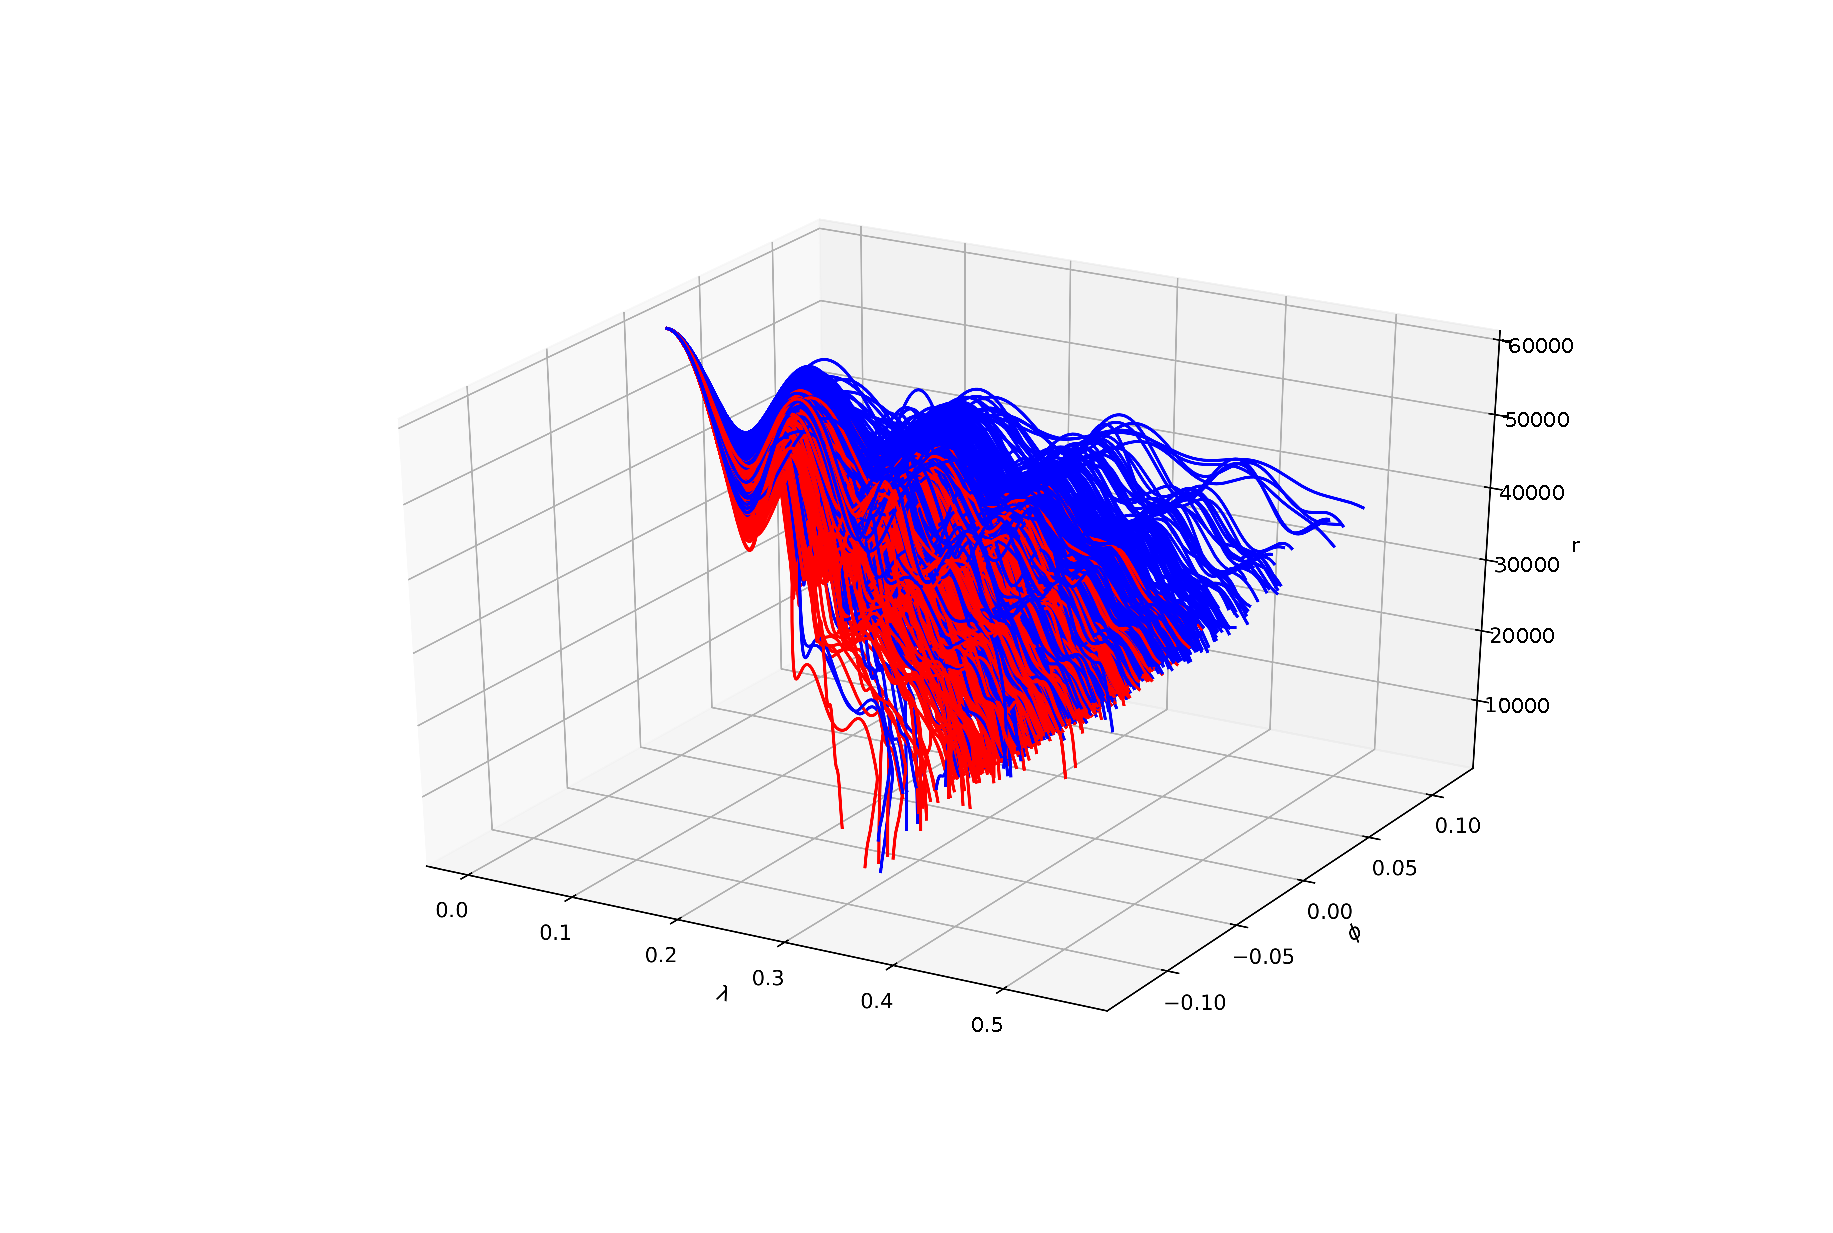
\includegraphics[width=1\linewidth]{Img/chapter7/3D-raw.eps}
\caption{高超声速飞行器轨迹三维图示}
\label{fig:hfvmixxxx}
\end{figure}

\begin{figure}
\centering
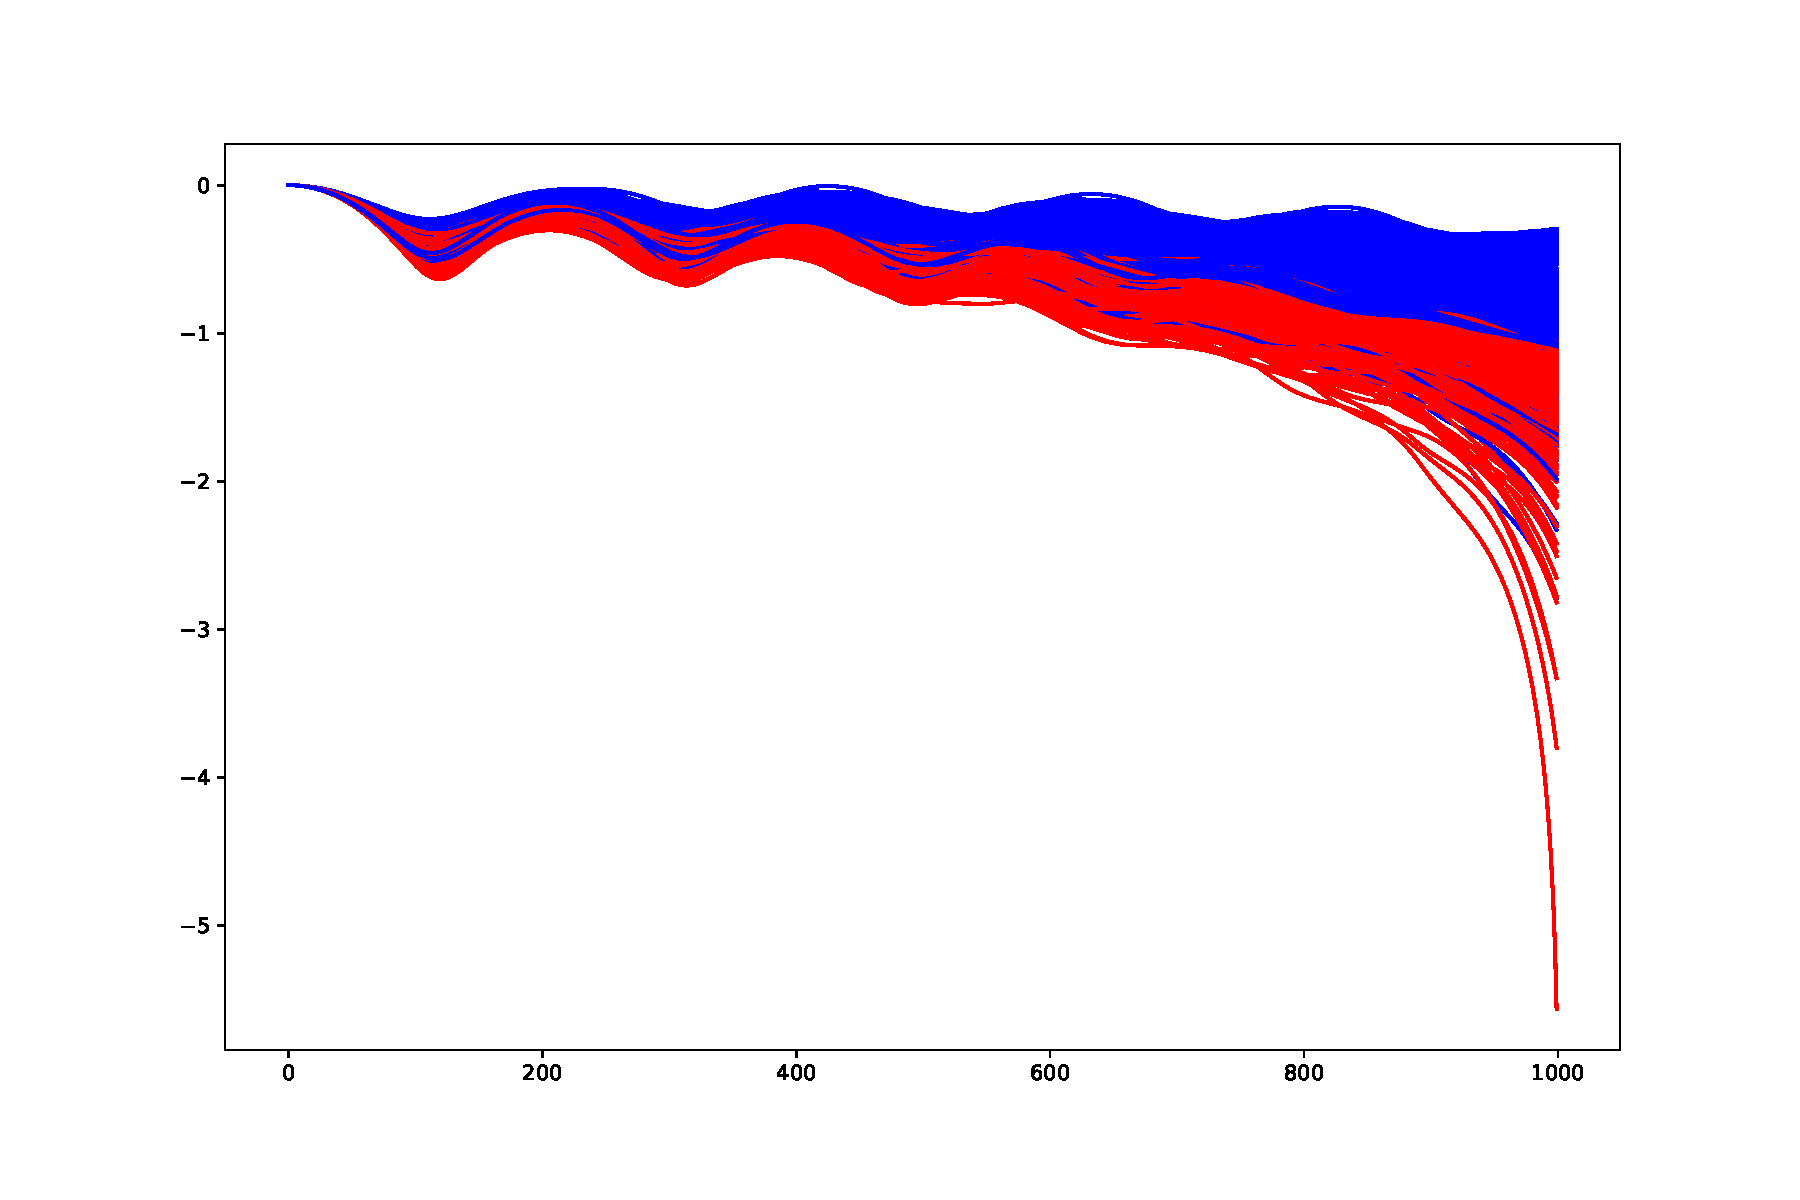
\includegraphics[width=1\linewidth]{Img/chapter7/log-return.eps}
\caption{高超声速飞行器轨迹坐标变换后图示}
\label{fig:hfvlog}
\end{figure}


\section{泛函数据分析一致性预测建模}
\label{sec:fda}
\subsection{泛函数据分析建模}

在本节开始, 我们将对泛函数据分析理论给出精炼的介绍. 对于经典模型, 直接地使用诸观测事实面临诸多的困难, 这些困难集中表现在下列若干方面: 首先, 对于处理复杂问题, 我们再也不能将观测视为直接的向量, 相反的, 我们所面对的经验数据一定是离散的随机变量, 这些随机变量理应被视为诸函数. 因此, 在这一层意义上可以确定传统基于统计学的各种方法都不能直接应用于处理这类问题. 因此, 当经验数据被视为“函数”后, 统计学家们提出的泛函数据分析方法为这类问题提供了一种解决方案, 针对泛函数据分析方法的详尽的介绍, 参见\citep{Ramsay2009} 和 \citep{Kokoszka2017}的著作.

泛函数据分析的常用方法是将原始数据映射至特征空间, 这些曲线的原始观测数据被压缩提取为主要特征, 即
\begin{align}\label{fdaform}
X_{n}(t) \in \mathbb{R}, n=1,2,\ldots,N, t = 1,\ldots,T,
\end{align}
其中, 这里 $N$ 是曲线的数目, $T$ 是观测时长.

为了简明起见, 在本文中我们所处理的泛函数据是按照下列表达式处理的, 即我们将原始观测分解至各个基函数上, 
\begin{align}\label{basisexpansion}
X_{n}(t) = \sum_{m=1}^{M}c_{nm}B_{m}(t), 1 \leq n \leq N,
\end{align}
其中, 这里$B_{m}$ 是先验确立的基函数, 例如可以选择$B$-样条基函数, 小波基函数, 或者傅里叶基函数, 这里 $c_{nm}$是所估计的系数. 表达式 (\ref{basisexpansion}) 反映的是这样一种思想, 即诸观测事实都是光滑函数, 并且这些光滑函数共享相同的形状属性同时可以通过$M$个基函数$B_{m}$的线性组合来近似, 其中这里的基函数数目$M$通常小于观测时长$T$. 如果诸观测轨迹的记录时间 $T$ 非常大, 例如在本文中我们的记录时间均大于 $1000$s, 那么采用基展开表达式 (\ref{basisexpansion}) 就可以将原始观测数据$X_{n}(t)$表征为由诸系数$c_{nm}$所确立的较小的组合. 对于每一条曲线 $X_{n}(t)$, 其都可以通过维数为$M$的列向量 $c_n = [c_{n1},c_{n2},\ldots,c_{nM}]^T$来表征. 这样一来, 直接观测获得的经验数据就被投射至指定的某数学空间. 需要注意的是,  泛函数据分析最关键的步骤是对所得到的的数据展开主成分分析, 以尽可能提取其关键特征. 在表达式(\ref{basisexpansion})中, 基函数$B_m$是固定的. 泛函主成分分析的思想就是寻找满足下列光滑条件的函数$\hat{v}_j$, 使得 $X_{n}(t) = \sum_{m=1}^{M}c_{nm}B_{m}(t)$ 可以表示为下列表达式:
\begin{align}
\label{functionalpca}
X_{n}(t) = \sum_{m=1}^{M}c_{nm}B_{m}(t) =  \sum_{j=1}^{p}\hat{\epsilon}_{nj}\hat{v}_{j}(t),
\end{align}
其中, 这里主成分数目$p$是远小于表达式(\ref{functionalpca})中的基函数数目$M$的. 所估计得到的泛函主成分 (Estimated Functional Principle Components, EFPC) $\hat{v}_j$都是将经验观测数据转变为泛函对象所得到的结果, 当基函数类型的选择被先验地确立后, 问题的核心其实就是确立主成分数目. 

对于分类问题设定, 通过泛函数据分析, 每条曲线$X_{n}(t)$被表征为估计得到的泛函主成分向量$\hat{\epsilon}_{n} = [\hat{\epsilon}_{n1},\hat{\epsilon}_{n2},...,\hat{\epsilon}_{np}]^T$, 而这里的主成分数目 $p$ 通常远小于比基函数数目 $M$. 我们将基于所得到的泛函主成分数据来展开模式识别算法并且为此提供有效的不确定性量化.

\subsection{底层超越算子建模}
\label{SVMs}
在本节我们简要介绍支持向量机 (Support Vector Machines, SVMs) 用于分类任务\citet{vapnik1995,vapnik1998,Vapnik2006}. 我们所处理的问题现在归约为二元分类问题, 这是经典的模式识别问题, 分类标签标记为-1 和 1. 我们的目标是当训练数据无法完全分开情形下, 如何通过容量控制使得机器达到最优的推广泛化能力 \citep{Cortes1995}. 

设训练数据集
\begin{align*}
(x_1,y_1),\ldots,(x_l,y_l), x \in \mathbb{R}^{n}, y \in \{-1,1\},
\end{align*}
无法通过一个超平面达到完全分开. 在这种情形下, 我们的目标是建构一个超平面, 其能够最小化错误数目. 为此, SVM引进非负松弛变量
\begin{align*}
\xi_1,\ldots,\xi_l.
\end{align*}
这样一来, 我们需要最小化下列泛函
\begin{align}
R(w,b) = \sum_{i=1}^{l}\xi_i,
\end{align}
其针对的约束条件是
\begin{align}
y_{i}((w,z_{i}) + b) \geq 1 - \xi_{i}, \xi_{i} \geq 0, i = 1,\ldots,l,
\end{align}
以及下列约束条件
\begin{align}
(w,w) \leq h.
\end{align}
其中, 这里的$h$是诸超平面集合的VC维度. $z$是输入数据$x$通过算子$z = \mathcal{F}x$对应的象空间.

为了求解这一问题, 我们需要寻找下列优化问题的拉格朗日乘子的鞍点
\begin{align}
L(w,b,\alpha,\beta,\gamma) = \sum_{i=1}^{l}\xi_{i}
- \frac{1}{2}\gamma((w,w) - h)
- \sum_{i=1}^{l}\alpha_{i}(y_{i}(w,w)+b)-1 + \xi_{i})
- \sum_{i=1}^{l}\beta_{i}\xi_{i},
\end{align}
(此优化问题是针对$w,b,\xi_{i}$取最小, 针对非负乘子$\alpha_{i},\beta_{i},\gamma$取最大). 最小化此拉格朗日乘子的参数必须满足下列条件
\begin{align*}
\frac{\partial L(w,b,\alpha,\beta,\gamma)}{\partial w} &= \gamma w - \sum_{i=1}^{l}\alpha_{i}y_{i}z_{i} = 0,\\
\frac{\partial L(w,b,\alpha,\beta,\gamma)}{\partial b} &= -\sum_{i=1}^{l}y_{i}\alpha_{i} = 0,\\
\frac{\partial L(w,b,\alpha,\beta,\gamma)}{\partial \xi_i} &= 1 - \alpha_{i} - \beta_{i} = 0.
\end{align*}
从这些条件中我们可以得到下列表达式
\begin{align}
&w = \frac{1}{\gamma}\sum_{i=1}^{l}\alpha_{i}y_{i}z_{i},\\
&\sum_{i=1}^{l}\alpha_{i}y_{i} = 0,\\
&\alpha_{i} + \beta_{i} = 1.
\end{align}
将这些表达式带入拉格朗日乘子, 我们得到下列泛函
\begin{align}
W(\alpha) = \sum_{i=1}^{l}\alpha_{i} - h\sqrt{\sum_{i,j=1}^{l}y_{i}y_{j}\alpha_{i}\alpha_{j}(z_{i},z_{j})},
\end{align}
其约束条件维
\begin{align}
\sum_{i=1}^{l}y_{i}\alpha_{i} = 0,
\end{align}
以及下列约束条件
\begin{align*}
0 \leq \alpha_{i} \leq 1, i=1,\ldots,l.
\end{align*}
通过求解此优化问题, 我们就能够得到模式识别问题的求解.

\subsection{归纳一致性预测算法建模}
\label{ICP}
为机器学习算法提供不确定量化是基于一致性预测展开的\citep{vovk2005algorithmic,2006Hedging,shafer08a}. 下列数据对
\begin{align*}
z_1,\ldots,z_l,
\end{align*}
假设随由相同的概率分布函数独立地生成的, 我们将$z_i = (x_i,y_i)$称之为\textsf{样本}. 每个样本$z_i$由其对象$x_{i}$和对应的标签$y_{i}$构成. 给定新的对象$x_{l+1}$, 我们的目标是预测其类别标签$y_{l+1}$. 在本节我们所处理的问题中, 所有的标准假设都是数据服从I.I.D假设. 我们先验地知道所有可能的类别标签数目$Y_1,\ldots,Y_{c}$. 从随机性的算法理论视角来看, 如果对于仅有一个扩展——这个“扩展”正就是给出的预测标签——的新序列, 得到的算法随机性度量是一个较小的值, 那么, 我们就能够基于给定的训练集$z_1,\ldots,z_{l}$, 为新对象$x_{l+1}$的标签$y_{l+1}$给出一个可信的集合预测, 即
\begin{align*}
(z_1,\ldots,z_{l},(x_{l+1},y)),y \in {Y_1,\ldots,Y_c},
\end{align*}
这样以来, 我们就能够输出对应 $y$ 的可信集合预测. \citet{Kolmogorov1963,MartinLf1966,Kolmogorov1968,Kolmogorov1983,Li2008} 为算法随机性理论给出了详细的讨论, 我们此处的一致性预测方法是对算法随机理论的直接应用. 具体来说, 基于\citet{MartinLf1966}, 函数$p: Z^{*} \rightarrow [0,1]$是针对I.I.D模型随机性的一个检测函数, 就是说这个函数满足如下的性质, 即如果
\begin{enumerate}
\item[1.] $\forall n \in \mathbb{N}, \forall \delta \in [0,1]$ 并且针对基于样本$Z$上的所有概率分布$P^{n}$, 都满足
\begin{align}
P^{n}\{z \in Z^{n}: p(z) \leq \delta \} \leq \delta,
\end{align}
\item[2.] $p$ 是半可计算函数.
\end{enumerate}
那么, 这样的函数就能够扮演随机性检测函数. 如果按照统计学的术语, 这样定义的随机性检测函数就大体上等同于$p$-值. 因此, 通过借助计算每个标签$Y_{j},j=1,\ldots,c$所对应的$p$-值, 我们就可以得到针对此序列的随机性检测度量, 我们将之记为 $p(Y_{j})$.

正如文献\citet{vovk2005algorithmic}所阐述的, 任何一致性预测输出结果都是精确有效的, 这就意味着, 任何一致性预测方法所产生的$p$-值都将是独立的, 并且严格服从$[0,1]$上的均匀分布. 关于一致性预测方法所产生的$p$-值是精确有效的这一陈述的证明, 参见\citet{vovk2005algorithmic}.

在具体应用中, 如果给定标签下序列计算得到的$p$-值小于某一给定的显著性水平$\alpha$, 例如$\alpha = 0.05$, 这意味着下列序列
\begin{align*}
((x_1,y_1),\ldots,(x_l,y_l),(x_{l+1},Y_j)),
\end{align*}
拒绝原假设. 也就是说, 拒绝“原序列是I.I.D序列”这一假设. 为了计算新添加了标签的样本与其他已收集样本由多么大的不同, 我们需要使用下列函数 $A_{n}: Z^{(n-1)} \times Z \rightarrow \mathbb{R},n=1,2,\ldots$,  此函数会为每个样本 $z_{i}$ 计算得到一个度量值, 即
\begin{align}
\label{alpha}
\alpha_{i} = A_{n}((z_1,\ldots,z_{i-1},z_{i+1},\ldots,z_{l}), z_{i}),
\end{align}
这一度量值指明了到底这一样本与已经分好类别的序列$(z_{1},\ldots,z_{i-1},z_{i+1},\ldots,z_{l})$有多么大的区分程度. 对于新的测试对象$x_{l+1}$, 因为我们先验地知道所有可能的类别标签 $Y_{j},j=1,\ldots,c$, 所以我们可以在每个可能的标签下, 借助任意的机器学习算法——我们将之称之为底层算法$D$\footnote{称之为“底层算法”是为了凸显一致性预测方法可以应用与任意的机器学习、神经网络、深度学习算法. 形象地说, 一致性预测能够为各种学习算法刷上一层有效的不确定量化量度.}——我们就可以计算此非一致测度得分, 即可得
\begin{align}
y_{l+1}^{Y_{j}} = D(x_{l+1}), j = 1,\ldots,c.
\end{align}
通过将计算得到的不相似程度排序, 我们就能够度量新预测类别到底与训练序列中的那些样本差异有多大
\footnote{我们的零假设是序列来自I.I.D.}
, 也就是说, 我们得到下列比较后的$p$-值,
\begin{align}\label{align:pvalue}
p(Y_{j}) = \frac{\#\{i=1,\ldots,l,l+1: \alpha_{i}^{(Y_j)} \geq \alpha_{l+1}^{(Y_{j})}\}}{l+1},j=1,\ldots,c.
\end{align}
当我们得到新对象$x_{l+1}$的预测值所对应的$p$-值$p(Y_{j}), j=1,\ldots,c$之后, 很自然地, 我们将最大的$p$-值视为此预测的可信度指标, 将1减去第二大$p$-值所得结果视为是此次预测的可信度度量.

我们在本文中考虑归纳框架下一致性预测(Inductive Conformal Prediction, ICP), 我们在采用SVM作为底层算法的同时, 还考虑将神经网络, 决策树和Boosting等算法作为底层算法, 并且对比各种算法之间的效果. 对于经验数据$z_{i} = (x_{i}, y_{i}), i = 1,2,\ldots, g$, 将之\textsf{随机切分}为两部分, 其中一部分作为训练数据\textsf{$Z_{\text{training}}$} = $\{z_{1},\ldots,z_{l}\}$, 另一部分作为测试数据\textsf{$Z_{\text{test}}$} = $\{z_{1+1},\ldots,z_{g}\}$. 对于训练数据集, 我们进一步将之切分为真正的训练集合 (the proper training set)\textsf{$Z_{\text{proper}}$} = $\{z_{1},\ldots,z_{m}\}$ 和校正集\textsf{$Z_{\text{calibration}}$} = $\{z_{m+1},\ldots,z_{l}\}$. 我们在真正训练集上得到学习模型, 然后在校验集合上计算非一致得分 (nonconformity scores), $p$-值, 并且得到测试集的一致性预测结果. 

对于校验数据集样本, 算法按照表达式(\ref{alpha})输出一致性预测概率值$y_{l+1}^{Y_{j}}$和其非一致得分. 对于测试样本, 根据底层算法得到其模型输出结果, 而其非一致得分和$p$-值的计算分别按照表达式Eq. (\ref{alpha})和表达式(\ref{align:pvalue})计算得到. 例如在本文中, 我们主要列举了置信水平分别为 99\%, 95\%, 90\%, 和 80\% 情况下的预测结果. 在具体的置信水平下, 我们计算得到$p$-值, 并且得到此置信水平下的有保证的分类结果. 图\ref{fig:flow}显示了一致性预测方法处理高超声速飞行器的整个步骤.

\begin{figure}
\centering
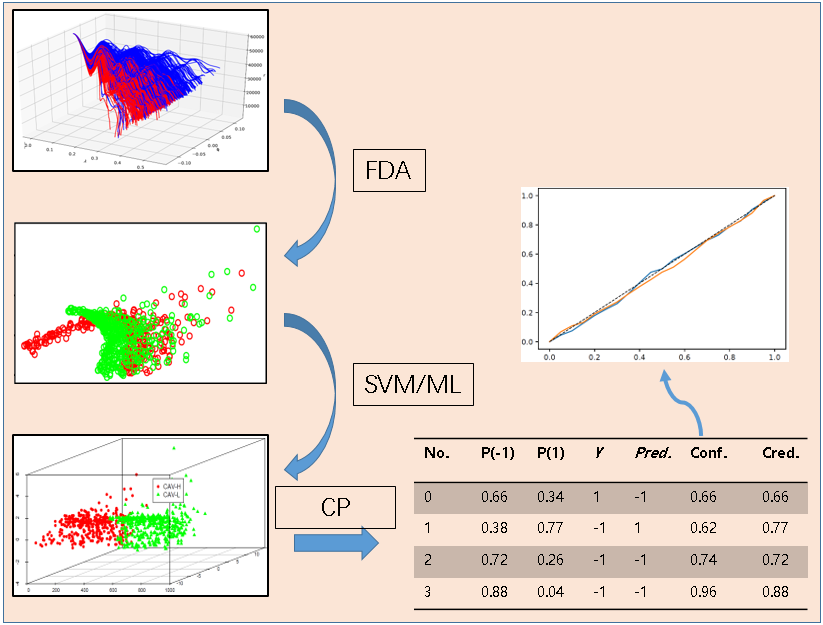
\includegraphics[width=.7\linewidth]{Img/chapter7/Flow.png}
\caption{高超声速飞行器轨迹分类的一致性预测方法图示}
\label{fig:flow}
\end{figure}

\section{结果与讨论}
\label{sec:results}

在本节我们详细描述利用一致性预测方法处理基于高超声速飞行器轨迹数据型号分类问题结果. 这里的轨迹数据是基于第\ref{sec:dynamic}节所介绍的动力学模型模拟得到的. 针对每一种机动模式, 我们模拟生成2400条轨迹数据, 并且通过先验地引入$B$-样条基函数作为建构泛函数据分析的基函数, 将经验观测数据转换为泛函数据对象后, 通过观测函数 $X_1, X_2, \ldots, X_{N}$ 确立估计主成分数目$p$. 最后, 我们将得到的特征数据按照2:1:1的关系\textsf{随机切分}为真实训练集, 校正集和测试集合, 并且利用真实训练数据集合构建分类学习算法.

借助底层学习算法——例如SVMs, Boosting和神经网络算法——我们计算序列$(z_1,\ldots,z_{l})$中每个样例$z_i=(x_{i},y_{i})$的非一致得分. 底层学习算法创建了一个预测决策规则 $D_{(z_1,\ldots,z_l)}$,  这一规则将为无标记的候选对象$x_{l+1}$映射一个预测标识 $\hat{y}_{l+1}$. 在训练过程中, 此规则是基于给定的序列给出预测标记$\hat{y}_{i} = D(x_{i})$, 给出的标签同时指认了样例$z_i$与序列中的其他样本到底有多么的相似; 这里的输出结果 $\hat{y}_{i}$ 得分越高, 表明其与序列中的其他样本越一致. 因此, 我们可以将输出得分的取反值(即 inverse probability)视为是非一致得分$\alpha_{i}$的度量 \citep{Aleksandrova2021}, 即
\begin{align}
\alpha_{i} = -\hat{y}_{i},
\end{align}
其中, 这里的非一致得分$\alpha_{i}$给出的是样本$z_{i}$的非一致性度量. 使用SVMs模型(我们采用默认参数, 即选择RBF作为核函数, 正则化参数$C$=1.0)作为底层算法. 在这里我们报告经过一致性预测方法增强后的SVMs算法 (即SVMs-CP)结果, 与此同时, 我们还采用Boosting, 神经网络算法 (Neural Networks, NN), Na{\"i}ve Bayes (NB) 以及逻辑回归 (Logistic Regression, LR) 和线性判别方法 (Linear Discriminant Analysis, LDA) 等传统统计方法作为底层算法. 所有的这些实验都由Python下的开源机器学习程序包$\mathtt{scikit-learn}$实现, 各类算法的参数均采用默认参数. 于此同时, 我们还比较了对于采用不同的基函数(例如采用傅里叶基函数)下泛函数据分析方法的推广能力. 

表\ref{tab:accuracy} 列出了这些比较的结果, 从表中我们可以看到, 采用不同的泛函数据分析基函数(比如我们比较了$B$-样条基函数与傅里叶基函数)不会对分类结果产生显著的改善. 这也正好应证了我们关于基函数选择的批判分析. 例如, 对于B-样条和傅里叶基函数, SVMs算法给出的分类准确率稳定在74\%左右, 决策树算法给出的分类准确率稳定在75\%左右. 但是各种机器学习算法(SVMs, 决策树, 提升算法Boosting和神经网络)比传统方法(朴素贝叶斯, 逻辑回归和线性判别法)都要优越.

对于一致性预测的具体例子而言, 不仅仅比较了分类的准确性, 我们同时也检验了$p$-值的品质, 通过比较 99\%, 95\%, 90\% 和 80\% 置信水平下的$p$-值分布, 我们可以看出, 一致性预测方法所得到的 $p$-值是有效的. 而为了报告一致性预测方法的结果, 我们需要将输出结果分为以下四种可能: 
\begin{enumerate}
\item[1.] $>1$(\%): 预测集合中元素个数大于1的数目所占的比例.
\item[2.] $=1$(\%): 预测集合中元素个数等于1的数目所占的比例.
\item[3.] $\emptyset$(\%): 预测集合为空集所占的比例.
\item[4.] Accuracy(\%): 正确预测所占的比例.
\end{enumerate}
需要说明的是, 对于集合预测的情形, 如果真实标签被预测的集合包含在内, 我们认为这样的预测结果是正确的. 我们的主要关切点是, 对于所预测的集合, 我们希望单个元素的集合预测数目所占的比重越大越好, 这就意味着, 虽然我们给出的是具有集合预测信息的结果, 但是因为预测结果中单元素集合数目占比很大, 这就表明我们的预测效率较高. 不仅如此, 我们还报告了单元素集合所占的比例以及根据一致性预测方法得到的预测准确度. 最后我们报告了预测结果为空集的情形所占比的比例, 我们希望这个比例值越小越好. 所有的这些信息都汇总在表\ref{tab:CP-methods}中. 从表中同时可以看到, 一致性预测方法所得到的准确率达到了理论要求的准确率, 因此, 从错误率控制的角度来看, 一致性预测方法是有效的.

为了确认可信度测量, 针对不同的底层算法(分别是SVM, Boosting, 神经网络方法, Na\"{i}ve Bayes, Logistic 回归和线性判别法), 我们都检查其预测的每个类别所对应的$p$-值的经验分布, 这些结果都列在图 \ref{fig:pvalue}中. 这些结果表明, 一致性预测方法所产生的的预测结果是有效的. 表\ref{tab:cp-svm}给出了SVMs作为底层算法, 经过一致性预测方法计算得到的不确定性度量的例子. 表\ref{tab:cp-svm} 的第一列是样本索引号, 表中其余列分别表示每个类别计算得到的$p$-值, 真实标签, 一致性预测标签 (CP-Lable), 置信度以及可信度. 可以确认的是, 不同于传统方法中仅仅报告不确定水平的汇总信息 (例如, 在传统方法中一般报告均方误差作为模型结果的评定准则), 利用一致性预测方法可以针对每个样本提供有效的不确定性度量. 

表\ref{tab:set-prediction-hfv}列出了从高超声速飞行器轨迹数据集合中挑选出来的样例 (这种挑选主要是为了说明集合预测的效果, 并没有选择性地挑选预测优质样本), 表中列出了不同类别下对应的$p$-值, 不同的显著性水平以及真实的类别标签. 表中的结果显示对于任意给定的显著性水平, 一致性预测方法都能够给出其所对应的集合预测结果.

\begin{table}[]
\centering
\caption{底层算法在不同基函数下准确度比较}
\label{tab:accuracy}
\begin{tabular}{@{}r|rr@{}}
\toprule
\multirow{2}{*}{底层算法} & \multicolumn{2}{r}{准确度(\%)} \\ \cmidrule(l){2-3}
		& B-spline        & Fourier        \\ \midrule
SVMs    & 74.71           & 74.71          \\
DT		& 75.37			& 72.05			 \\
Boosting& 73.38           & 74.38          \\
NN      & 72.55           & 74.04          \\
NB      & 58.74           & 57.07          \\
LR      & 46.59           & 46.92          \\
LDA     & 46.59           & 46.92          \\ \bottomrule
\end{tabular}
\end{table}

%\begin{figure}
%\centering
%  \includegraphics[width=.7\linewidth]{Img/chapter7/CAV-HL-FDA.eps}
%  \caption{The functional data analysis plots of different maneuver models of the hypersonic flight vehicle.}
%  \label{fig:hfvfda}
%\end{figure}
%
%\begin{figure}
%\centering
%  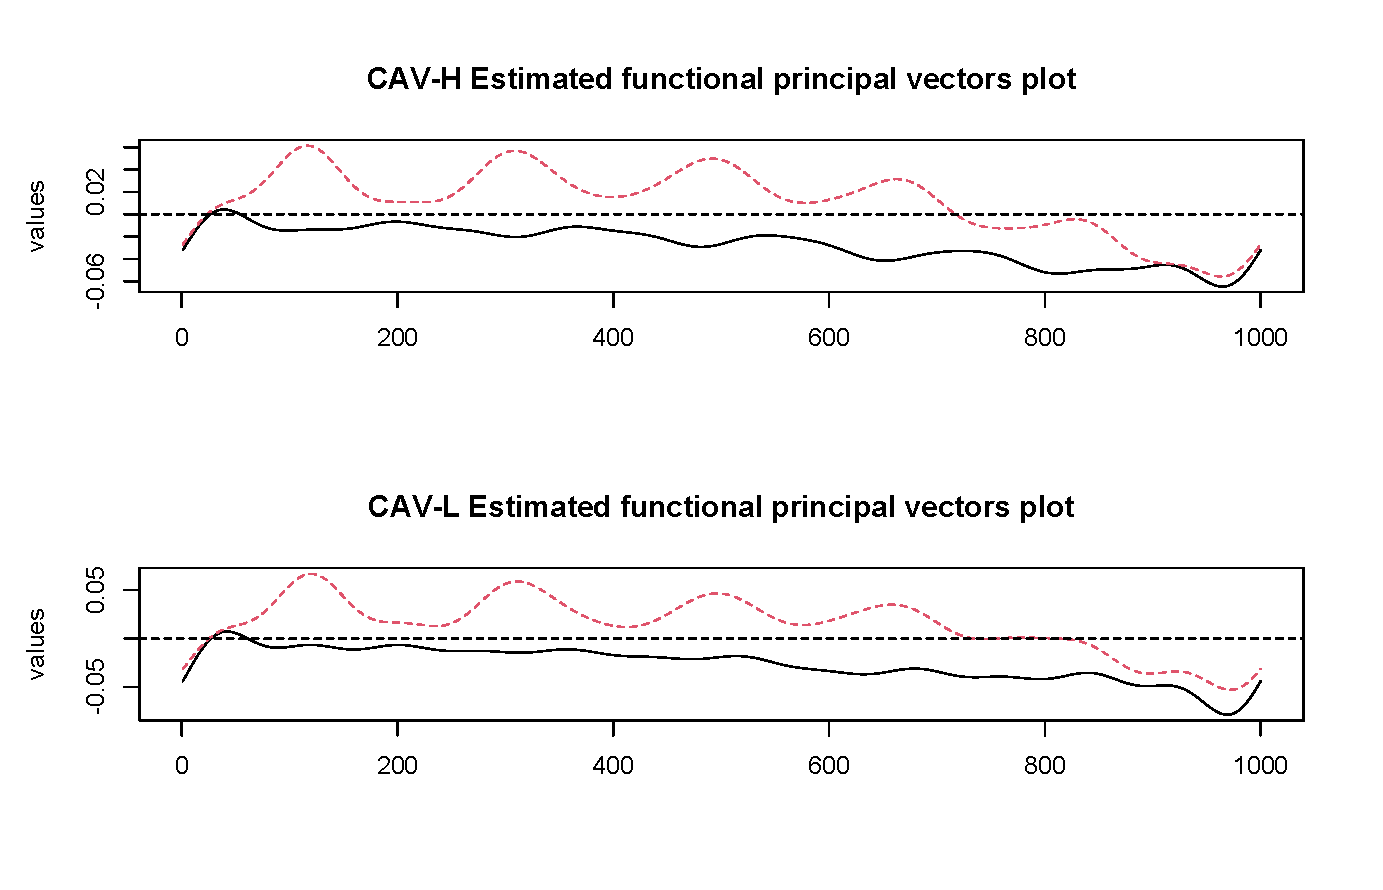
\includegraphics[width=.7\linewidth]{Img/chapter7/CAV-HL-PCA.eps}
%  \caption{The estimated principal components plots of different maneuver models of the hypersonic flight vehicle.}
%  \label{fig:hfvpca}
%\end{figure}

\begin{table}[]
\centering
\caption{各种底层算法的一致性预测增强后准确度比较}
\label{tab:CP-methods}
\begin{tabular}{@{}rccccc@{}}
\toprule
Algorithm &
  \multicolumn{1}{l}{1-$\epsilon$} &
  \multicolumn{1}{l}{准确率(\%)} &
  \multicolumn{1}{l}{=1(\%)} &
  \multicolumn{1}{l}{\textgreater{}1(\%)} &
  \multicolumn{1}{l}{$\emptyset$(\%)} \\ \midrule
\multirow{4}{*}{SVMs-CP}     & 99\% & 99.66  & 18.14 & 81.86 & 0.00  \\
                          & 95\% & 94.16  & 40.10 & 59.90 & 0.00 \\
                          & 90\% & 90.65  & 52.25 & 47.75 & 0.00 \\
                          & 80\% & 81.70  & 79.03 & 20.97 & 0.00 \\ \midrule
\multirow{4}{*}{DT-CP}       & 99\% & 99.67  & 27.45 & 72.54 & 0.00 \\
                          & 95\% & 96.17  & 44.93 & 55.07 & 0.00 \\
                          & 90\% & 92.20  & 57.90 & 42.10 & 0.00 \\
                          & 80\% & 82.68  & 82.03 & 18.00 & 0.00 \\ \midrule
\multirow{4}{*}{Boosting-CP} & 99\% & 99.83  & 8.49 & 91.51 & 0.00  \\
                          & 95\% & 96.88  & 25.96 & 70.04 & 0.00 \\
                          & 90\% & 91.50  & 49.25 & 50.75 & 0.00 \\
                          & 80\% & 82.89  & 76.71 & 23.29 & 0.00 \\ \midrule
\multirow{4}{*}{NN-CP}       & 99\% & 100  & 7.82 & 92.17 & 0.00 \\
                          & 95\% & 95.32  & 34.44 & 65.56 & 0.00 \\
                          & 90\% & 92.12  & 46.42 & 53.58 & 0.00 \\
                          & 80\% & 80.50  & 81.70 & 18.30 & 0.00 \\ \midrule
\multirow{4}{*}{NB-CP}       & 99\% & 99.49  & 4.50 & 95.50 & 0.00  \\
                          & 95\% & 96.00  & 15.14 & 84.85 & 0.00 \\
                          & 90\% & 92.66  & 24.63 & 75.37 & 0.00 \\
                          & 80\% & 80.56  & 47.59 & 52.41 & 0.00 \\ \midrule
\multirow{4}{*}{LR-CP}       & 99\% & 99.67  & 4.66 & 95.34 & 0.00  \\
                          & 95\% & 94.31  & 15.31 & 84.69 & 0.00 \\
                          & 90\% & 89.17  & 22.96 & 77.04 & 0.00 \\
                          & 80\% & 78.80 & 39.10 & 60.89 & 0.00 \\ \midrule
\multirow{4}{*}{LDA-CP}      & 99\% & 99.67  & 4.66 & 95.34 & 0.00  \\
                          & 95\% & 94.31  & 15.31 & 84.69 & 0.00 \\
                          & 90\% & 89.17  & 22.96 & 77.04 & 0.00 \\
                          & 80\% & 78.80 & 39.10 & 60.89 & 0.00 \\ \bottomrule
\end{tabular}
\end{table}

%========================subfigure
\begin{figure}[h]
\centering
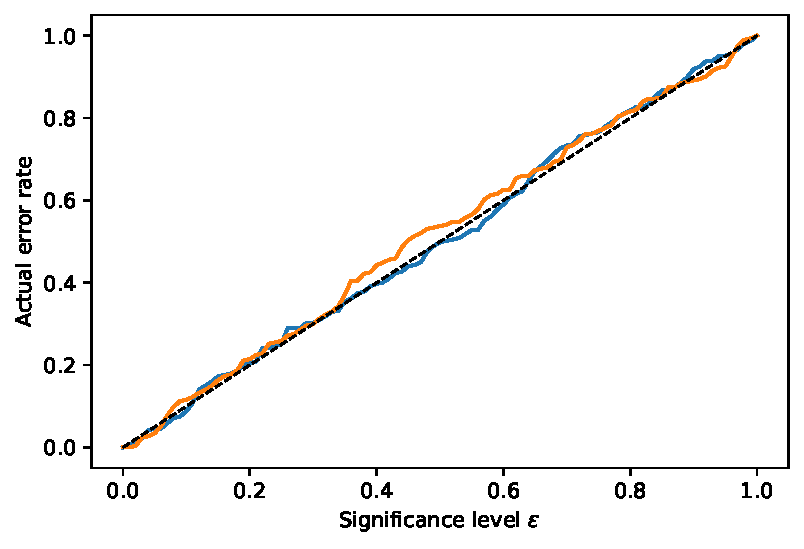
\includegraphics[width=.4\linewidth]{Img/chapter7/svm_validity.pdf}
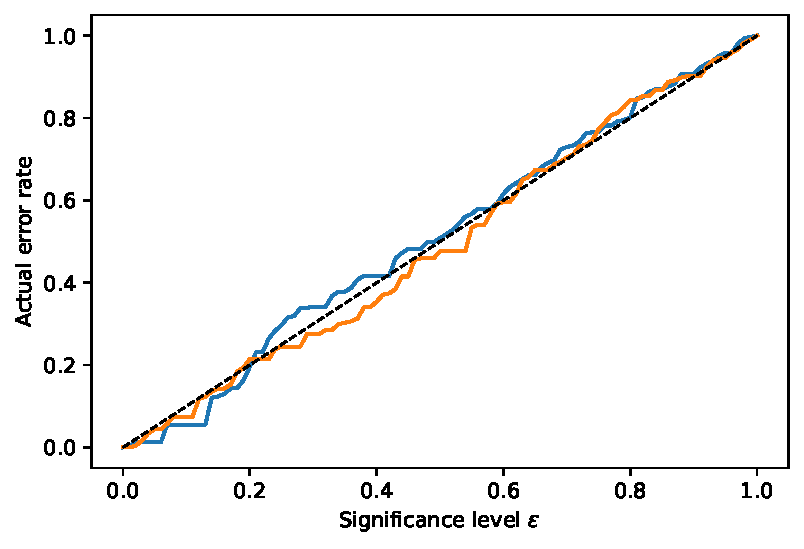
\includegraphics[width=.4\linewidth]{Img/chapter7/boosting_validity.pdf}
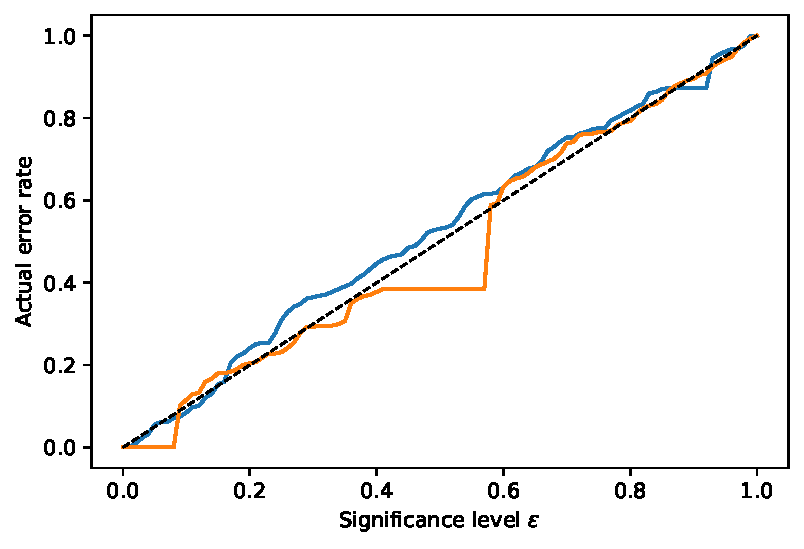
\includegraphics[width=.4\linewidth]{Img/chapter7/mlp_validity.pdf}
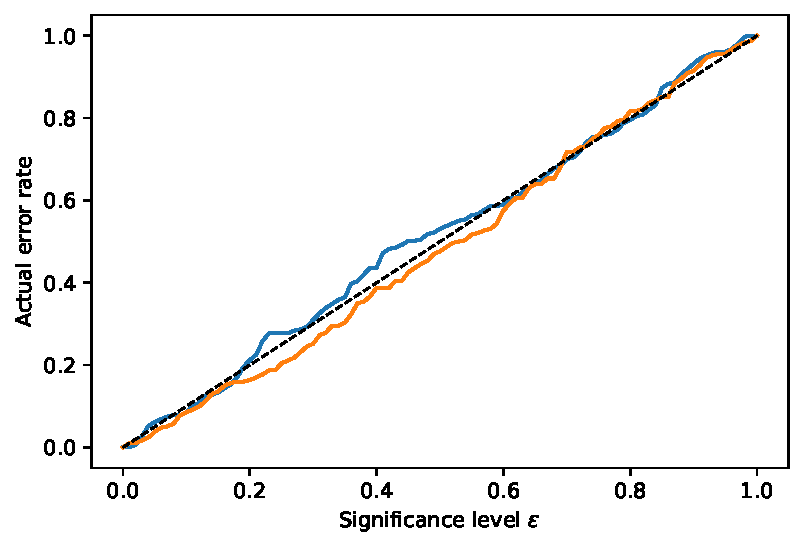
\includegraphics[width=.4\linewidth]{Img/chapter7/naive_validity.pdf}
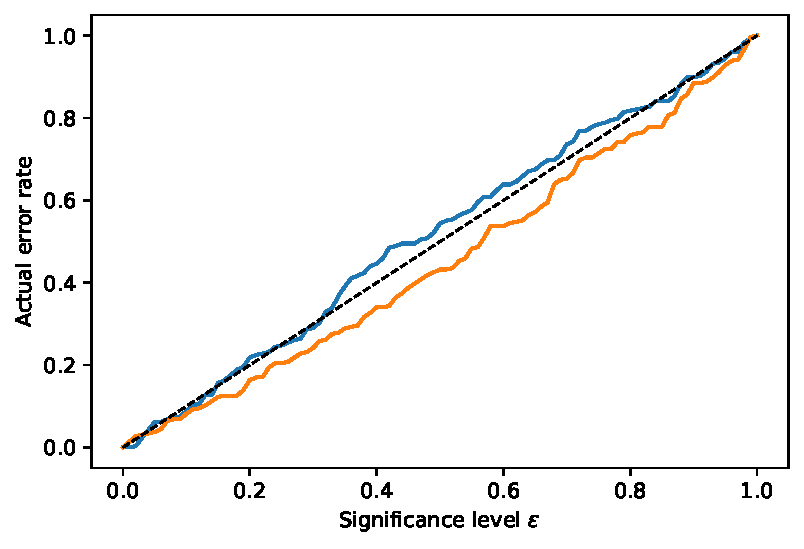
\includegraphics[width=.4\linewidth]{Img/chapter7/logistic_validity.pdf}
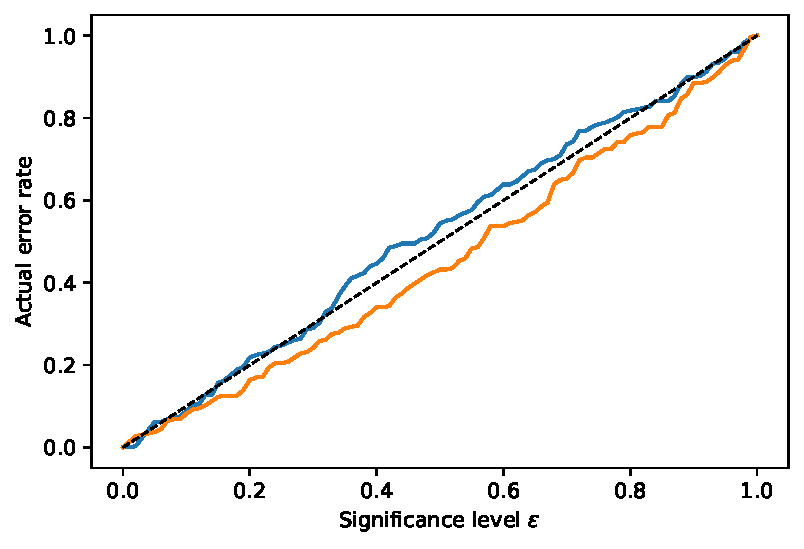
\includegraphics[width=.4\linewidth]{Img/chapter7/lda_validity.pdf}
\caption{不同底层算法对应$p$-值的经验分布}
\label{fig:pvalue}
\end{figure}





% Please add the following required packages to your document preamble:
% \usepackage{booktabs}
\begin{table}[]
\centering
\caption{SVMs-CP方法的不确定度量结果}
\label{tab:cp-svm}
\begin{tabular}{@{}ccccccc@{}}
\toprule
\#  & -1        & 1        & 真实标签 & SVMs-CP标签 & 置信度 & 可信度 \\ \midrule
0	&0.872483	&0.613115	&-1	&-1	&0.386885	&0.872483\\
1	&0.845638	&0.619672	&-1	&-1	&0.380328	&0.845638\\
2	&0.184564	&0.960656	&1	&1	&0.815436	&0.960656\\
3	&0.825503	&0.655738	&-1	&-1	&0.344262	&0.825503\\
4	&0.755034	&0.718033	&-1	&-1	&0.281967	&0.755034\\
5	&0.446309	&0.849180	&1	&1	&0.553691	&0.849180\\
6	&0.580537	&0.777049	&1	&1	&0.419463	&0.777049\\
7	&0.711409	&0.724590	&1	&1	&0.288591	&0.724590\\
8	&0.963087	&0.419672	&-1	&-1	&0.580328	&0.963087\\
9	&0.436242	&0.852459	&1	&1	&0.563758	&0.852459 \\
10	&0.718121	&0.721311	&-1	&1	&0.281879	&0.721311\\
11	&0.718121	&0.721311	&-1	&1	&0.281879	&0.721311\\
12	&0.718121	&0.721311	&-1	&1	&0.281879	&0.721311\\
\bottomrule
\multicolumn{1}{l}{} & \multicolumn{1}{l}{} & \multicolumn{1}{l}{} & \multicolumn{1}{l}{} & \multicolumn{1}{l}{} & \multicolumn{1}{l}{} & \multicolumn{1}{l}{}
\end{tabular}
\end{table}

% Please add the following required packages to your document preamble:
% \usepackage{booktabs}
% \usepackage{lscape}
\begin{landscape}
\begin{table}[]
\centering
\caption{SVMs-CP方法的集合预测结果}
\label{tab:set-prediction-hfv}
\begin{tabular}{@{}cccccccccccccccccc@{}}
\toprule
\# & -1 & 1 & 0.01 & 0.05 & 0.1 & 0.15 & 0.2 & 0.25 & 0.5 & 0.75 & 0.8 & 0.85 & 0.9 & 0.95 & 0.99 & 1 & 真实标签 \\ \midrule
1 & 0.382550 & 0.773770 & {[}-1, 1{]} & {[}-1, 1{]} & {[}-1, 1{]} & {[}-1, 1{]} & {[}-1, 1{]} & {[}-1, 1{]} & {[}1{]} & {[}1{]} & {[}{]} & {[}{]} & {[}{]} & {[}{]} & {[}{]} & {[}{]} & -1 \\
2 & 0.721477 & 0.245902 & {[}-1, 1{]} & {[}-1, 1{]} & {[}-1, 1{]} & {[}-1, 1{]} & {[}-1, 1{]} & {[}-1{]} & {[}-1{]} & {[}{]} & {[}{]} & {[}{]} & {[}{]} & {[}{]} & {[}{]} & {[}{]} & -1 \\
3 & 0.882550 & 0.036066 & {[}-1, 1{]} & {[}-1{]} & {[}-1{]} & {[}-1{]} & {[}-1{]} & {[}-1{]} & {[}-1{]} & {[}-1{]} & {[}-1{]} & {[}-1{]} & {[}{]} & {[}{]} & {[}{]} & {[}{]} & -1 \\
4 & 0.053691 & 0.940984 & {[}-1, 1{]} & {[}-1, 1{]} & {[}1{]} & {[}1{]} & {[}1{]} & {[}1{]} & {[}1{]} & {[}1{]} & {[}1{]} & {[}1{]} & {[}1{]} & {[}{]} & {[}{]} & {[}{]} & -1 \\
5 & 0.120805 & 0.901639 & {[}-1, 1{]} & {[}-1, 1{]} & {[}-1, 1{]} & {[}1{]} & {[}1{]} & {[}1{]} & {[}1{]} & {[}1{]} & {[}1{]} & {[}1{]} & {[}1{]} & {[}{]} & {[}{]} & {[}{]} & -1 \\
6 & 0.087248 & 0.934426 & {[}-1, 1{]} & {[}-1, 1{]} & {[}1{]} & {[}1{]} & {[}1{]} & {[}1{]} & {[}1{]} & {[}1{]} & {[}1{]} & {[}1{]} & {[}1{]} & {[}{]} & {[}{]} & {[}{]} & -1 \\
7 & 0.174497 & 0.875410 & {[}-1, 1{]} & {[}-1, 1{]} & {[}-1, 1{]} & {[}-1, 1{]} & {[}1{]} & {[}1{]} & {[}1{]} & {[}1{]} & {[}1{]} & {[}1{]} & {[}{]} & {[}{]} & {[}{]} & {[}{]} & -1 \\
8 & 0.013423 & 0.993443 & {[}-1, 1{]} & {[}1{]} & {[}1{]} & {[}1{]} & {[}1{]} & {[}1{]} & {[}1{]} & {[}1{]} & {[}1{]} & {[}1{]} & {[}1{]} & {[}1{]} & {[}1{]} & {[}{]} & 1 \\
9 & 0.194631 & 0.865574 & {[}-1, 1{]} & {[}-1, 1{]} & {[}-1, 1{]} & {[}-1, 1{]} & {[}1{]} & {[}1{]} & {[}1{]} & {[}1{]} & {[}1{]} & {[}1{]} & {[}{]} & {[}{]} & {[}{]} & {[}{]} & -1 \\
105	&0.137584	&0.881967	&[0, 1]	&[0, 1]	&[0, 1]	&[1]	&[1]	&[1]	&[1]	&[1]	&[1]	&[1]	&[]	&[]	&[]	&[]	&0 \\
427	&0.140940	&0.881967	&[0, 1]	&[0, 1]	&[0, 1]	&[1]	&[1]	&[1]	&[1]	&[1]	&[1]	&[1]	&[]	&[]	&[]	&[]	&0 \\
415	&0.046980	&0.944262	&[0, 1]	&[1]	&[1]	&[1]	&[1]	&[1]	&[1]	&[1]	&[1]	&[1]	&[1]&[]	&[]	&[]	&0 \\
37	&0.127517	&0.891803	&[0, 1]	&[0, 1]	&[0, 1]	&[1]	&[1]	&[1]	&[1]	&[1]	&[1]	&[1]	&[]	&[]	&[]	&[]	&0 \\
115	&0.127517	&0.891803	&[0, 1]	&[0, 1]	&[0, 1]	&[1]	&[1]	&[1]	&[1]	&[1]	&[1]	&[1]	&[]	&[]	&[]	&[]	&1 \\
487 & 0.016779 & 0.983607 & {[}0, 1{]} & {[}1{]} & {[}1{]} & {[}1{]} & {[}1{]} & {[}1{]} & {[}1{]} & {[}1{]} & {[}1{]} & {[}1{]} & {[}1{]} & {[}1{]} & {[}{]} & {[}{]} & 1 \\
284 & 0.003356 & 1.000000 & {[}1{]} & {[}1{]} & {[}1{]} & {[}1{]} & {[}1{]} & {[}1{]} & {[}1{]} & {[}1{]} & {[}1{]} & {[}1{]} & {[}1{]} & {[}1{]} & {[}1{]} & {[}{]} & 1 \\
378 & 0.114094 & 0.904918 & {[}0, 1{]} & {[}0, 1{]} & {[}0, 1{]} & {[}1{]} & {[}1{]} & {[}1{]} & {[}1{]} & {[}1{]} & {[}1{]} & {[}1{]} & {[}1{]} & {[}{]} & {[}{]} & {[}{]} & 1 \\
\bottomrule
\end{tabular}
\end{table}
\end{landscape}


\section{本章小结}
\label{sec:conclusion}
在本节中, 我们基于高超声速飞行器轨迹数据, 为高超声速飞行器型号的辨识提供一种概率有保证的分类方法, 并且为每个预测样本都提供了其预测结果的不确定性度量. 针对每个预测样本, 我们提供了两种度量指标, 分别是置信度和可信度说. 与传统统计方法指导下的不确定性度量方法不同的是, 一致性预测方法所产生的不确定性度量结果不需要任何分布假设, 是一种无分布假设的不确定性量化方法. 

本文所给出的方法是基于泛函数据分析方法而展开的. 首先, 我们介绍了泛函数据分析的基本理论并且借助泛函数据分析工具, 将原始观测数据映射至先验指定的特征空间, 然后在特征空间构建模式识别算法, 利用SVMs等底层算法得到高超声速飞行器的型号分类. 

对于泛函数据分析, 我们也探究了不同基函数对分类结果的影响. 我们给出了$B$-样条基函数和傅里叶基函数下的结果对比. 最终的结果表明, 基函数的先验选择对预测性能的改变微乎其微. 需要额外强调的是, 有别于传统统计, 我们所提出的方法关注的是每个样本的不确定性量化结果, 对于汇总的量化结果并不是我们特别关注的对象.

更进一步, 我们引进一致性预测方法为底层学习算法的输出给出有效的不确定性量化分析. 所有的不确定性量化结果都是基于底层算法的输出展开并且不需要任何分布假设. 与此同时, 我们还将一致性预测方法输出$p$-值的经验分布作了检验, 结果表明对于任意的一致性预测方法, 其给出的$p$-值都是精确有效的.